
\newcolumntype{A} { > {\centering\arraybackslash } p{35pt} }
\newcolumntype{D} { > {\centering\arraybackslash } p{66pt} }
\newcolumntype{L} { > {\centering\arraybackslash } p{15pt} }
\newcolumntype{C} { > {\centering\arraybackslash } p{22pt} }
\newcolumntype{R} { > {\centering\arraybackslash } p{33pt} }

% BANNER INFO
\newcommand{\CharacterNameValue}{}
\newcommand{\ClassValue}{}
\newcommand{\SubclassValue}{}
\newcommand{\BackgroundValue}{}
\newcommand{\PlayerNameValue}{}
\newcommand{\SpeciesValue}{}
\newcommand{\AlignmentValue}{} %not in the banner
\newcommand{\XPValue}{}
\newcommand{\LevelValue}{}

\newcommand{\CharacterName}[1]{\renewcommand{\CharacterNameValue}{#1}}
\newcommand{\Class}[1]{\renewcommand{\ClassValue}{#1}}
\newcommand{\Subclass}[1]{\renewcommand{\SubclassValue}{#1}}
\newcommand{\Background}[1]{\renewcommand{\BackgroundValue}{#1}}
\newcommand{\PlayerName}[1]{\renewcommand{\PlayerNameValue}{#1}}
\newcommand{\Species}[1]{\renewcommand{\SpeciesValue}{#1}}
\newcommand{\Alignment}[1]{\renewcommand{\AlignmentValue}{#1}}
\newcommand{\Level}[1]{\renewcommand{\LevelValue}{#1}}
\newcommand{\XP}[1]{\renewcommand{\XPValue}{#1}}


%all white
	\newrgbcolor{SDia1}{1 1 1}%
	\newrgbcolor{SDia2}{1 1 1}%
	\newrgbcolor{SDia3}{1 1 1}%


	\newrgbcolor{FDia1}{1 1 1}%
	\newrgbcolor{FDia2}{1 1 1}%
	\newrgbcolor{FDia3}{1 1 1}%

\newcommand{\DeathSaves}[2]{%
	\ifnum#1>0 \newrgbcolor{SDia1}{0.235 0.361 0.216}\fi
	\ifnum#1>1 \newrgbcolor{SDia2}{0.235 0.361 0.216}\fi
	\ifnum#1>2 \newrgbcolor{SDia3}{0.235 0.361 0.216}\fi
%black diamonds
	\ifnum#2>0 \newrgbcolor{FDia1}{0.502 0.235 0.204}\fi
	\ifnum#2>1 \newrgbcolor{FDia2}{0.502 0.235 0.204}\fi
	\ifnum#2>2 \newrgbcolor{FDia3}{0.502 0.235 0.204}\fi
}

\newcommand{\TransparentImages}[1]{%
	\ifthenelse{\equal{#1}{1}}{%
	\newbox\chara
        \savebox\chara{
\includegraphics[scale=0.2]{template/images/a_tt.png}}

        \newbox\charb
        \savebox\charb{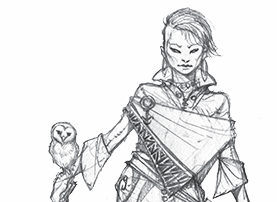
\includegraphics[scale=0.175]{template/images/b_tt.png}}

        \newbox\charc
        \savebox\charc{
\includegraphics[scale=0.21]{template/images/c_tt.png}}

        \newbox\chard
        \savebox\chard{
\includegraphics[scale=0.19]{template/images/d_tt.png}}

        \newbox\chare
        \savebox\chare{
\includegraphics[scale=0.14]{template/images/e_tt.png}}
	}{%
	\newbox\chara
        \savebox\chara{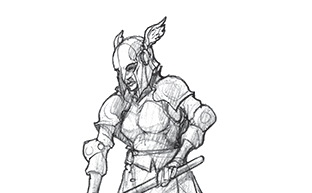
\includegraphics[scale=0.2]{template/images/a_t.png}}

        \newbox\charb
        \savebox\charb{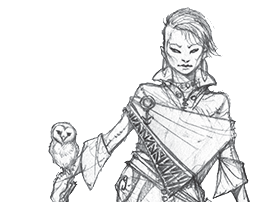
\includegraphics[scale=0.175]{template/images/b_t.png}}

        \newbox\charc
        \savebox\charc{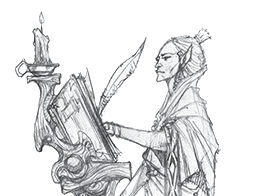
\includegraphics[scale=0.21]{template/images/c_t.png}}

        \newbox\chard
        \savebox\chard{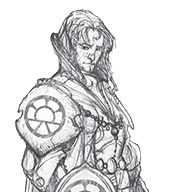
\includegraphics[scale=0.19]{template/images/d_t.png}}

        \newbox\chare
        \savebox\chare{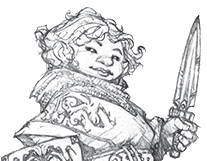
\includegraphics[scale=0.14]{template/images/e_t.png}}
	}
}

% PROFICIENCY ETC
\newcommand{\InspirationValue}{}
\newcommand{\ProficiencyValue}{}
\newcommand{\PerceptionValue}{}

\newcommand{\Inspiration}[1]{\renewcommand{\InspirationValue}{#1}}
\newcommand{\Proficiency}[1]{\renewcommand{\ProficiencyValue}{#1}}
\newcommand{\Perception}[1]{\renewcommand{\PerceptionValue}{#1}}

% ABILITY SCORES
\newcommand{\StrengthScoreValue}{}
\newcommand{\DexterityScoreValue}{}
\newcommand{\ConstitutionScoreValue}{}
\newcommand{\IntelligenceScoreValue}{}
\newcommand{\WisdomScoreValue}{}
\newcommand{\CharismaScoreValue}{}

\newcommand{\StrengthScore}[1]{\renewcommand{\StrengthScoreValue}{#1}}
\newcommand{\DexterityScore}[1]{\renewcommand{\DexterityScoreValue}{#1}}
\newcommand{\ConstitutionScore}[1]{\renewcommand{\ConstitutionScoreValue}{#1}}
\newcommand{\IntelligenceScore}[1]{\renewcommand{\IntelligenceScoreValue}{#1}}
\newcommand{\WisdomScore}[1]{\renewcommand{\WisdomScoreValue}{#1}}
\newcommand{\CharismaScore}[1]{\renewcommand{\CharismaScoreValue}{#1}}

% ABILITY MODIFIERS
\newcommand{\StrengthModifierValue}{}
\newcommand{\DexterityModifierValue}{}
\newcommand{\ConstitutionModifierValue}{}
\newcommand{\IntelligenceModifierValue}{}
\newcommand{\WisdomModifierValue}{}
\newcommand{\CharismaModifierValue}{}

\newcommand{\StrengthModifier}[1]{\renewcommand{\StrengthModifierValue}{#1}}
\newcommand{\DexterityModifier}[1]{\renewcommand{\DexterityModifierValue}{#1}}
\newcommand{\ConstitutionModifier}[1]{\renewcommand{\ConstitutionModifierValue}{#1}}
\newcommand{\IntelligenceModifier}[1]{\renewcommand{\IntelligenceModifierValue}{#1}}
\newcommand{\WisdomModifier}[1]{\renewcommand{\WisdomModifierValue}{#1}}
\newcommand{\CharismaModifier}[1]{\renewcommand{\CharismaModifierValue}{#1}}

% SAVING THROWS
\newcommand{\StrengthSavingThrowModifierValue}{}
\newcommand{\DexteritySavingThrowModifierValue}{}
\newcommand{\ConstitutionSavingThrowModifierValue}{}
\newcommand{\IntelligenceSavingThrowModifierValue}{}
\newcommand{\WisdomSavingThrowModifierValue}{}
\newcommand{\CharismaSavingThrowModifierValue}{}

\newcommand{\StrengthSavingThrowModifier}[1]{\renewcommand{\StrengthSavingThrowModifierValue}{#1}}
\newcommand{\DexteritySavingThrowModifier}[1]{\renewcommand{\DexteritySavingThrowModifierValue}{#1}}
\newcommand{\ConstitutionSavingThrowModifier}[1]{\renewcommand{\ConstitutionSavingThrowModifierValue}{#1}}
\newcommand{\IntelligenceSavingThrowModifier}[1]{\renewcommand{\IntelligenceSavingThrowModifierValue}{#1}}
\newcommand{\WisdomSavingThrowModifier}[1]{\renewcommand{\WisdomSavingThrowModifierValue}{#1}}
\newcommand{\CharismaSavingThrowModifier}[1]{\renewcommand{\CharismaSavingThrowModifierValue}{#1}}

%SKILLS
\newcommand{\AcrobaticsSkillModifierValue}{}
\newcommand{\AnimalHandlingSkillModifierValue}{}
\newcommand{\ArcanaSkillModifierValue}{}
\newcommand{\AthleticsSkillModifierValue}{}
\newcommand{\DeceptionSkillModifierValue}{}
\newcommand{\HistorySkillModifierValue}{}
\newcommand{\InsightSkillModifierValue}{}
\newcommand{\IntimidationSkillModifierValue}{}
\newcommand{\InvestigationSkillModifierValue}{}
\newcommand{\MedicineSkillModifierValue}{}
\newcommand{\NatureSkillModifierValue}{}
\newcommand{\PerceptionSkillModifierValue}{}
\newcommand{\PerformanceSkillModifierValue}{}
\newcommand{\PersuasionSkillModifierValue}{}
\newcommand{\ReligionSkillModifierValue}{}
\newcommand{\SleightOfHandSkillModifierValue}{}
\newcommand{\StealthSkillModifierValue}{}
\newcommand{\SurvivalSkillModifierValue}{}

\newcommand{\AcrobaticsSkillModifier}[1]{\renewcommand{\AcrobaticsSkillModifierValue}{#1}}
\newcommand{\AnimalHandlingSkillModifier}[1]{\renewcommand{\AnimalHandlingSkillModifierValue}{#1}}
\newcommand{\ArcanaSkillModifier}[1]{\renewcommand{\ArcanaSkillModifierValue}{#1}}
\newcommand{\AthleticsSkillModifier}[1]{\renewcommand{\AthleticsSkillModifierValue}{#1}}
\newcommand{\DeceptionSkillModifier}[1]{\renewcommand{\DeceptionSkillModifierValue}{#1}}
\newcommand{\HistorySkillModifier}[1]{\renewcommand{\HistorySkillModifierValue}{#1}}
\newcommand{\InsightSkillModifier}[1]{\renewcommand{\InsightSkillModifierValue}{#1}}
\newcommand{\IntimidationSkillModifier}[1]{\renewcommand{\IntimidationSkillModifierValue}{#1}}
\newcommand{\InvestigationSkillModifier}[1]{\renewcommand{\InvestigationSkillModifierValue}{#1}}
\newcommand{\MedicineSkillModifier}[1]{\renewcommand{\MedicineSkillModifierValue}{#1}}
\newcommand{\NatureSkillModifier}[1]{\renewcommand{\NatureSkillModifierValue}{#1}}
\newcommand{\PerceptionSkillModifier}[1]{\renewcommand{\PerceptionSkillModifierValue}{#1}}
\newcommand{\PerformanceSkillModifier}[1]{\renewcommand{\PerformanceSkillModifierValue}{#1}}
\newcommand{\PersuasionSkillModifier}[1]{\renewcommand{\PersuasionSkillModifierValue}{#1}}
\newcommand{\ReligionSkillModifier}[1]{\renewcommand{\ReligionSkillModifierValue}{#1}}
\newcommand{\SleightOfHandSkillModifier}[1]{\renewcommand{\SleightOfHandSkillModifierValue}{#1}}
\newcommand{\StealthSkillModifier}[1]{\renewcommand{\StealthSkillModifierValue}{#1}}
\newcommand{\SurvivalSkillModifier}[1]{\renewcommand{\SurvivalSkillModifierValue}{#1}}

% BATTLE STATS
\newcommand{\ArmorClassValue}{}
\newcommand{\InitiativeValue}{}
\newcommand{\SpeedValue}{}
\newcommand{\MaxHitPointsValue}{}
\newcommand{\CurrentHitPointsValue}{}
\newcommand{\TemporaryHitPointsValue}{}
\newcommand{\MaxHitDiceValue}{}
\newcommand{\SpentHitDiceValue}{}

\newcommand{\ArmorClass}[1]{\renewcommand{\ArmorClassValue}{#1}}
\newcommand{\Initiative}[1]{\renewcommand{\InitiativeValue}{#1}}
\newcommand{\Speed}[1]{\renewcommand{\SpeedValue}{#1}}
\newcommand{\MaxHitPoints}[1]{\renewcommand{\MaxHitPointsValue}{#1}}
\newcommand{\CurrentHitPoints}[1]{\renewcommand{\CurrentHitPointsValue}{#1}}
\newcommand{\TemporaryHitPoints}[1]{\renewcommand{\TemporaryHitPointsValue}{#1}}
\newcommand{\MaxHitDice}[1]{\renewcommand{\MaxHitDiceValue}{#1}}
\newcommand{\SpentHitDice}[1]{\renewcommand{\SpentHitDiceValue}{#1}}

% MONEY
\newcommand{\CPValue}{}
\newcommand{\SPValue}{}
\newcommand{\GPValue}{}
\newcommand{\EPValue}{}
\newcommand{\PPValue}{}

\newcommand{\CP}[1]{\renewcommand{\CPValue}{#1}}
\newcommand{\SP}[1]{\renewcommand{\SPValue}{#1}}
\newcommand{\GP}[1]{\renewcommand{\GPValue}{#1}}
\newcommand{\EP}[1]{\renewcommand{\EPValue}{#1}}
\newcommand{\PP}[1]{\renewcommand{\PPValue}{#1}}

\newcommand{\EquipmentValue}{}

% EQUIPMENT TRAINING & PROFICIENCIES

%Weapons
\newcommand{\WeaponsProficienciesValue}{}
\newcommand{\WeaponsProficiencies}[1]{\renewcommand{\WeaponsProficienciesValue}{#1}}

%Tools
\newcommand{\ToolsProficienciesValue}{}
\newcommand{\ToolsProficiencies}[1]{\renewcommand{\ToolsProficienciesValue}{#1}}

% WEAPONS GENERATOR COMMAND 
% --- added 4th information (notes) --- has to be blank or will cause error
%TODO: make 4th command optional for cross-compatibility
\newcommand{\WeaponsHeld}{}

\makeatletter
\newcommand\AddWeapon[4]{%
	\g@addto@macro\WeaponsHeld{%
	\\[5.85pt]%
	\begin{fitbox}{94pt}{10pt}{\normalsize}\entryfont \textcolor{text-color}{#1}\end{fitbox}&
	\begin{fitbox}{35pt}{10pt}{\normalsize}\entryfont \textcolor{text-color}{#2}\end{fitbox} &
	\begin{fitbox}{66pt}{10pt}{\normalsize}\entryfont \textcolor{text-color}{#3}\end{fitbox}&
	\begin{fitbox}{110pt}{10pt}{\normalsize}\entryfont \textcolor{text-color}{#4}\end{fitbox}
	}
}
\makeatother

% MAGIC ITEM COMMAND
\newcommand{\MagicItemsAttuned}{}

% Farben initial: alle weiß
\newrgbcolor{MIA1}{1 1 1}
\newrgbcolor{MIA2}{1 1 1}
\newrgbcolor{MIA3}{1 1 1}

% Zähler für Magic-Item-Zeilen
\newcount\MIARow
\MIARow=0

% Optional: Reset-Makro, z.B. vor einer neuen Liste
\newcommand{\MagicItemsReset}{%
  \MIARow=0\relax
  \colorlet{MIA1}{white}%
  \colorlet{MIA2}{white}%
  \colorlet{MIA3}{white}%
}

\makeatletter
\newcommand\AddMagicItem[2]{%
  % Zeilennummer hochzählen
  \advance\MIARow by 1\relax

  % Wenn in dieser Zeile in Spalte 1 eine 1 steht,
  % setze die passende MIA-Farbe auf schwarz:
  \ifnum\MIARow=1
    \ifnum#1=1\relax \colorlet{MIA1}{black}\fi
  \fi
  \ifnum\MIARow=2
    \ifnum#1=1\relax \colorlet{MIA2}{black}\fi
  \fi
  \ifnum\MIARow=3
    \ifnum#1=1\relax \colorlet{MIA3}{black}\fi
  \fi

  % ursprüngliches Verhalten beibehalten: Zeile anhängen
  \g@addto@macro\MagicItemsAttuned{%
    \\[6.4pt]%
    &
    \begin{fitbox}{145pt}{10pt}{\normalsize}\entryfont
      \textcolor{text-color}{#2}%
    \end{fitbox}%
  }%
}
\makeatother



%% SPELL GENERATOR COMMAND 
%% Thinking about 6 inputs <Level><Name><Cast Time><Range><CRM><Notes>
% --- Set all Colors to blue ---
\newcommand{\InitSpellColors}{%
  \multido{\n=1+1}{30}{%
  \begingroup
      % Name to text
      \edef\thisC{C\n}%
      \edef\thisR{R\n}%
      \edef\thisM{M\n}%
      % define every color as an RGB color (atm "white")
      \expandafter\newrgbcolor\expandafter{\thisC}{1 1 1}%
      \expandafter\newrgbcolor\expandafter{\thisR}{1 1 1}%
      \expandafter\newrgbcolor\expandafter{\thisM}{1 1 1}%
    \endgroup
	}%
}
\InitSpellColors %call command once before creating the spells


% --- Row-Counter, Marker-Store, Getter ---
\newcount\SpellRow
\SpellRow=0
\newcommand{\SpellRowStep}{\advance\SpellRow by 1\relax}
\newcommand{\SpellRowReset}{\SpellRow=0\relax}

% --- Marker per row --- 
\newcommand{\SpellMarkerStore}[1]{%
  \expandafter\gdef\csname SpellMarker@\the\SpellRow\endcsname{#1}%
}
\newcommand{\SpellMarkerGet}[1]{\csname SpellMarker@#1\endcsname}

% --- color logic per row (#1 = row number) ---
\makeatletter
\newcommand{\MakeSpellFlagColors}[1]{%
  \edef\Marker{\romannumeral-`0\SpellMarkerGet{#1}}%
  \edef\nC{C#1}\edef\nR{R#1}\edef\nM{M#1}%
  \expandafter\colorlet\expandafter{\nC}{white}%
  \expandafter\colorlet\expandafter{\nR}{white}%
  \expandafter\colorlet\expandafter{\nM}{white}%
  \IfSubStr{\Marker}{C}{\expandafter\colorlet\expandafter{\nC}{black}}{}%
  \IfSubStr{\Marker}{R}{\expandafter\colorlet\expandafter{\nR}{black}}{}%
  \IfSubStr{\Marker}{M}{\expandafter\colorlet\expandafter{\nM}{black}}{}%
}
\makeatother

% --- spell table for player-input ---
\newcommand{\SpellsReady}{}

% \AddSpellReady{lvl}{name}{cast}{range}{marker(CRM)}{effect}
\makeatletter
\newcommand\AddSpellReady[6]{%
  \SpellRowStep
  \SpellMarkerStore{#5}% remember 5. column
  \MakeSpellFlagColors{\the\SpellRow}% create colors for the row
  \g@addto@macro\SpellsReady{%
    \\[5.85pt]%
    \entryfont\textcolor{text-color}{#1} &
    \begin{fitbox}{100pt}{10pt}{\normalsize}\entryfont\textcolor{text-color}{#2}\end{fitbox} &
    \entryfont\textcolor{text-color}{#3} &
    \entryfont\textcolor{text-color}{#4} &
    \entryfont\textcolor{text-color}{} & %not used anymore, #5 for the letters :)
    \begin{fitbox}{80pt}{10pt}{\normalsize}\entryfont\textcolor{text-color}{#6}\end{fitbox}%
  }%
}

%% note: counter has to go up, but no markers
\newcommand\AddSpellNote[1]{%
  \SpellRowStep
  \expandafter\gdef\csname SpellMarker@\the\SpellRow\endcsname{}% empty marker
  \MakeSpellFlagColors{\the\SpellRow}% set C/R/M of the row to yellow
  \g@addto@macro\SpellsReady{%
    \\[5.85pt]%
    \multicolumn{4}{c}{%
      \begin{fitbox}{195pt}{10pt}{\footnotesize}\centering
        \entryfont\textcolor{text-color}{#1}%
      \end{fitbox}}&&%
  }%
}


\makeatother


%old, replaced (maybe include it into each other, to get cross-compatibility)
\newcommand{\FeaturesTraitsValue}{}
\newcommand{\OtherProficienciesLanguagesValue}{}
%not sure
\newcommand{\AttacksAdditionalValue}{}

\newcommand{\LanguagesValue}{}
\newcommand{\Languages}[1]{\renewcommand{\LanguagesValue}{#1}}

% CLASS FEATURES
\newcommand{\ClassFeaturesValue}{}
\newcommand{\ClassFeatures}[1]{\renewcommand{\ClassFeaturesValue}{#1}}

% SPECIES TRAITS
\newcommand{\SpecialTraitsValue}{}
\newcommand{\SpecialTraits}[1]{\renewcommand{\SpecialTraitsValue}{#1}}

% FEATS
\newcommand{\FeatsValue}{}
\newcommand{\Feats}[1]{\renewcommand{\FeatsValue}{#1}}

%not sure
\newcommand{\OtherProficienciesLanguages}[1]{\renewcommand{\OtherProficienciesLanguagesValue}{\raggedright#1}}
\newcommand{\AttacksAdditional}[1]{\renewcommand{\AttacksAdditionalValue}{#1}}
\newcommand{\Equipment}[1]{\renewcommand{\EquipmentValue}{#1}}

%old, replaced (maybe include it into each other, to get cross-compatibility)
%\newcommand{\FeaturesTraits}[1]{\renewcommand{\FeaturesTraitsValue}{#1}}


% APPEARANCE
\newcommand{\AgeValue}{}
\newcommand{\HeightValue}{}
\newcommand{\WeightValue}{}
\newcommand{\EyesValue}{}
\newcommand{\SkinValue}{}
\newcommand{\HairValue}{}
\newcommand{\CharacterAppearanceValue}{}
\newcommand{\AppearanceValue}{\CharacterAppearanceValue \par Age:~\AgeValue,\par Height:~\HeightValue,\par  Eyes:~\EyesValue,\par Skin:~\SkinValue,\par Hair:~\HairValue 
}


\newcommand{\Age}[1]{\renewcommand{\AgeValue}{#1}}
\newcommand{\Height}[1]{\renewcommand{\HeightValue}{#1}}
\newcommand{\Weight}[1]{\renewcommand{\WeightValue}{#1}}
\newcommand{\Eyes}[1]{\renewcommand{\EyesValue}{#1}}
\newcommand{\Skin}[1]{\renewcommand{\SkinValue}{#1}}
\newcommand{\Hair}[1]{\renewcommand{\HairValue}{#1}}
\newcommand{\Appearance}[1]{\renewcommand{\AppearanceValue}{#1}}
\newcommand{\CharacterAppearance}[1]{\renewcommand{\CharacterAppearanceValue}{#1}}

% PERSONALITY
\newcommand{\PersonalityTraitsValue}{}
\newcommand{\IdealsValue}{}
\newcommand{\BondsValue}{}
\newcommand{\FlawsValue}{}

\newcommand{\PersonalityTraits}[1]{\renewcommand{\PersonalityTraitsValue}{#1}}
\newcommand{\Ideals}[1]{\renewcommand{\IdealsValue}{#1}}
\newcommand{\Bonds}[1]{\renewcommand{\BondsValue}{#1}}
\newcommand{\Flaws}[1]{\renewcommand{\FlawsValue}{#1}}


% background

\newcommand{\AdditionalFeaturesAndTraitsValue}{}
\newcommand{\CharacterbackgroundValue}{}
\newcommand{\TreasureValue}{}
\newcommand{\AlliesAndOrganizationsValue}{}
\newcommand{\OrganizationNameValue}{}
\newcommand{\BackstoryValue}{\PersonalityTraitsValue \par \IdealsValue \par \BondsValue \par \FlawsValue \par \vspace{1em}
\AdditionalFeaturesAndTraitsValue \par 
\CharacterbackgroundValue \par 
\TreasureValue \par 
\AlliesAndOrganizationsValue \par 
\OrganizationNameValue \par 

}


\newcommand{\AdditionalFeaturesAndTraits}[1]{\renewcommand{\AdditionalFeaturesAndTraitsValue}{#1}}
\newcommand{\Characterbackground}[1]{\renewcommand{\CharacterbackgroundValue}{#1}}
\newcommand{\Treasure}[1]{\renewcommand{\TreasureValue}{#1}}
\newcommand{\AlliesAndOrganizations}[1]{\renewcommand{\AlliesAndOrganizationsValue}{#1}}
\newcommand{\OrganizationName}[1]{\renewcommand{\OrganizationNameValue}{#1}}
\newcommand{\Backstory}[1]{\renewcommand{\BackstoryValue}{#1}}

% SPELL MODIFIERS
\newcommand{\SpellcastingClassValue}{}
\newcommand{\SpellcastingAbilityValue}{}
\newcommand{\SpellcastingModifierValue}{}
\newcommand{\SpellSaveDCValue}{}
\newcommand{\SpellAttackBonusValue}{}

\newcommand{\SpellcastingClass}[1]{\renewcommand{\SpellcastingClassValue}{#1}}
\newcommand{\SpellcastingAbility}[1]{\renewcommand{\SpellcastingAbilityValue}{#1}}
\newcommand{\SpellcastingModifier}[1]{\renewcommand{\SpellcastingModifierValue}{#1}}
\newcommand{\SpellSaveDC}[1]{\renewcommand{\SpellSaveDCValue}{#1}}
\newcommand{\SpellAttackBonus}[1]{\renewcommand{\SpellAttackBonusValue}{#1}}



% TOTAL SPELL SLOTS
\newcommand{\FirstLevelSpellSlotsTotalValue}{}
\newcommand{\SecondLevelSpellSlotsTotalValue}{}
\newcommand{\ThirdLevelSpellSlotsTotalValue}{}
\newcommand{\FourthLevelSpellSlotsTotalValue}{}
\newcommand{\FifthLevelSpellSlotsTotalValue}{}
\newcommand{\SixthLevelSpellSlotsTotalValue}{}
\newcommand{\SeventhLevelSpellSlotsTotalValue}{}
\newcommand{\EighthLevelSpellSlotsTotalValue}{}
\newcommand{\NinthLevelSpellSlotsTotalValue}{}

\newcommand{\FirstLevelSpellSlotsTotal}[1]{\renewcommand{\FirstLevelSpellSlotsTotalValue}{#1}}
\newcommand{\SecondLevelSpellSlotsTotal}[1]{\renewcommand{\SecondLevelSpellSlotsTotalValue}{#1}}
\newcommand{\ThirdLevelSpellSlotsTotal}[1]{\renewcommand{\ThirdLevelSpellSlotsTotalValue}{#1}}
\newcommand{\FourthLevelSpellSlotsTotal}[1]{\renewcommand{\FourthLevelSpellSlotsTotalValue}{#1}}
\newcommand{\FifthLevelSpellSlotsTotal}[1]{\renewcommand{\FifthLevelSpellSlotsTotalValue}{#1}}
\newcommand{\SixthLevelSpellSlotsTotal}[1]{\renewcommand{\SixthLevelSpellSlotsTotalValue}{#1}}
\newcommand{\SeventhLevelSpellSlotsTotal}[1]{\renewcommand{\SeventhLevelSpellSlotsTotalValue}{#1}}
\newcommand{\EighthLevelSpellSlotsTotal}[1]{\renewcommand{\EighthLevelSpellSlotsTotalValue}{#1}}
\newcommand{\NinthLevelSpellSlotsTotal}[1]{\renewcommand{\NinthLevelSpellSlotsTotalValue}{#1}}

% EXPENDED SPELL SLOTS
\newcommand{\FirstLevelSpellSlotsExpendedValue}{}
\newcommand{\SecondLevelSpellSlotsExpendedValue}{}
\newcommand{\ThirdLevelSpellSlotsExpendedValue}{}
\newcommand{\FourthLevelSpellSlotsExpendedValue}{}
\newcommand{\FifthLevelSpellSlotsExpendedValue}{}
\newcommand{\SixthLevelSpellSlotsExpendedValue}{}
\newcommand{\SeventhLevelSpellSlotsExpendedValue}{}
\newcommand{\EighthLevelSpellSlotsExpendedValue}{}
\newcommand{\NinthLevelSpellSlotsExpendedValue}{}

\newcommand{\FirstLevelSpellSlotsExpended}[1]{\renewcommand{\FirstLevelSpellSlotsExpendedValue}{#1}}
\newcommand{\SecondLevelSpellSlotsExpended}[1]{\renewcommand{\SecondLevelSpellSlotsExpendedValue}{#1}}
\newcommand{\ThirdLevelSpellSlotsExpended}[1]{\renewcommand{\ThirdLevelSpellSlotsExpendedValue}{#1}}
\newcommand{\FourthLevelSpellSlotsExpended}[1]{\renewcommand{\FourthLevelSpellSlotsExpendedValue}{#1}}
\newcommand{\FifthLevelSpellSlotsExpended}[1]{\renewcommand{\FifthLevelSpellSlotsExpendedValue}{#1}}
\newcommand{\SixthLevelSpellSlotsExpended}[1]{\renewcommand{\SixthLevelSpellSlotsExpendedValue}{#1}}
\newcommand{\SeventhLevelSpellSlotsExpended}[1]{\renewcommand{\SeventhLevelSpellSlotsExpendedValue}{#1}}
\newcommand{\EighthLevelSpellSlotsExpended}[1]{\renewcommand{\EighthLevelSpellSlotsExpendedValue}{#1}}
\newcommand{\NinthLevelSpellSlotsExpended}[1]{\renewcommand{\NinthLevelSpellSlotsExpendedValue}{#1}}


% --- Spell Slots ---
% Level 1
\newcommand{\FirstLevelSpellSlotsValue}{}
%all white
	\newrgbcolor{1Dia1}{1 1 1}%
	\newrgbcolor{1Dia2}{1 1 1}%
	\newrgbcolor{1Dia3}{1 1 1}%
	\newrgbcolor{1Dia4}{1 1 1}%

\newcommand{\FirstLevelSpellSlots}[2]{%
	\renewcommand{\FirstLevelSpellSlotsValue}{#1}%
%black diamonds
	\ifnum#2>0 \newrgbcolor{1Dia1}{0 0 0}\fi
	\ifnum#2>1 \newrgbcolor{1Dia2}{0 0 0}\fi
	\ifnum#2>2 \newrgbcolor{1Dia3}{0 0 0}\fi
	\ifnum#2>3 \newrgbcolor{1Dia4}{0 0 0}\fi
}


% Level 2
\newcommand{\SecondLevelSpellSlotsValue}{}
% all white
\newrgbcolor{2Dia1}{1 1 1}%
\newrgbcolor{2Dia2}{1 1 1}%
\newrgbcolor{2Dia3}{1 1 1}%

\newcommand{\SecondLevelSpellSlots}[2]{%
  \renewcommand{\SecondLevelSpellSlotsValue}{#1}% Gesamtwert speichern
  % black diamonds
  \ifnum#2>0 \newrgbcolor{2Dia1}{0 0 0}\fi
  \ifnum#2>1 \newrgbcolor{2Dia2}{0 0 0}\fi
  \ifnum#2>2 \newrgbcolor{2Dia3}{0 0 0}\fi
}

% Level 3
\newcommand{\ThirdLevelSpellSlotsValue}{}
% all white
\newrgbcolor{3Dia1}{1 1 1}%
\newrgbcolor{3Dia2}{1 1 1}%
\newrgbcolor{3Dia3}{1 1 1}%

\newcommand{\ThirdLevelSpellSlots}[2]{%
  \renewcommand{\ThirdLevelSpellSlotsValue}{#1}%
  % black diamonds
  \ifnum#2>0 \newrgbcolor{3Dia1}{0 0 0}\fi
  \ifnum#2>1 \newrgbcolor{3Dia2}{0 0 0}\fi
  \ifnum#2>2 \newrgbcolor{3Dia3}{0 0 0}\fi
}

% Level 4
\newcommand{\ForthLevelSpellSlotsValue}{} % (Schreibweise aus deiner Vorlage beibehalten)
% all white
\newrgbcolor{4Dia1}{1 1 1}%
\newrgbcolor{4Dia2}{1 1 1}%
\newrgbcolor{4Dia3}{1 1 1}%

\newcommand{\ForthLevelSpellSlots}[2]{%
  \renewcommand{\ForthLevelSpellSlotsValue}{#1}%
  % black diamonds
  \ifnum#2>0 \newrgbcolor{4Dia1}{0 0 0}\fi
  \ifnum#2>1 \newrgbcolor{4Dia2}{0 0 0}\fi
  \ifnum#2>2 \newrgbcolor{4Dia3}{0 0 0}\fi
}

% Level 5
\newcommand{\FifthLevelSpellSlotsValue}{}
% all white
\newrgbcolor{5Dia1}{1 1 1}%
\newrgbcolor{5Dia2}{1 1 1}%
\newrgbcolor{5Dia3}{1 1 1}%

\newcommand{\FifthLevelSpellSlots}[2]{%
  \renewcommand{\FifthLevelSpellSlotsValue}{#1}%
  % black diamonds
  \ifnum#2>0 \newrgbcolor{5Dia1}{0 0 0}\fi
  \ifnum#2>1 \newrgbcolor{5Dia2}{0 0 0}\fi
  \ifnum#2>2 \newrgbcolor{5Dia3}{0 0 0}\fi
}

% Level 6
\newcommand{\SixthLevelSpellSlotsValue}{}
% all white
\newrgbcolor{6Dia1}{1 1 1}%
\newrgbcolor{6Dia2}{1 1 1}%

\newcommand{\SixthLevelSpellSlots}[2]{%
  \renewcommand{\SixthLevelSpellSlotsValue}{#1}%
  % black diamonds
  \ifnum#2>0 \newrgbcolor{6Dia1}{0 0 0}\fi
  \ifnum#2>1 \newrgbcolor{6Dia2}{0 0 0}\fi
}

% Level 7
\newcommand{\SeventhLevelSpellSlotsValue}{}
% all white
\newrgbcolor{7Dia1}{1 1 1}%
\newrgbcolor{7Dia2}{1 1 1}%

\newcommand{\SeventhLevelSpellSlots}[2]{%
  \renewcommand{\SeventhLevelSpellSlotsValue}{#1}%
  % black diamonds
  \ifnum#2>0 \newrgbcolor{7Dia1}{0 0 0}\fi
  \ifnum#2>1 \newrgbcolor{7Dia2}{0 0 0}\fi
}

% Level 8
\newcommand{\EighthLevelSpellSlotsValue}{}
% all white
\newrgbcolor{8Dia1}{1 1 1}%

\newcommand{\EighthLevelSpellSlots}[2]{%
  \renewcommand{\EighthLevelSpellSlotsValue}{#1}%
  % black diamond
  \ifnum#2>0 \newrgbcolor{8Dia1}{0 0 0}\fi
}

% Level 9
\newcommand{\NinthLevelSpellSlotsValue}{}
% all white
\newrgbcolor{9Dia1}{1 1 1}%

\newcommand{\NinthLevelSpellSlots}[2]{%
  \renewcommand{\NinthLevelSpellSlotsValue}{#1}%
  % black diamond
  \ifnum#2>0 \newrgbcolor{9Dia1}{0 0 0}\fi
}


% PROFICIENCY COLOR CHANGES
\newrgbcolor{strengthproficiency}{1 1 1}
\newrgbcolor{strengthproficiencyhalf}{1 1 1}

\newcommand{\StrengthProficiency}[1]{
	\ifthenelse{\equal{#1}{Proficient}}{
		\colorlet{strengthproficiency}{proficiency-marker-color} \colorlet{strengthproficiencyhalf}{proficiency-marker-color}}{}
	\ifthenelse{\equal{#1}{Half}}{
		\colorlet{strengthproficiencyhalf}{proficiency-marker-color}}{}
	\ifthenelse{\equal{#1}{Expert}}{
		\colorlet{strengthproficiency}{expert-proficiency-marker-color} \colorlet{strengthproficiencyhalf}{expert-proficiency-marker-color}}{}
}

\newrgbcolor{dexterityproficiency}{1 1 1}
\newrgbcolor{dexterityproficiencyhalf}{1 1 1}

\newcommand{\DexterityProficiency}[1]{
	\ifthenelse{\equal{#1}{Proficient}}{
		\colorlet{dexterityproficiency}{proficiency-marker-color} \colorlet{dexterityproficiencyhalf}{proficiency-marker-color}}{}
	\ifthenelse{\equal{#1}{Half}}{
		\colorlet{dexterityproficiencyhalf}{proficiency-marker-color}}{}
	\ifthenelse{\equal{#1}{Expert}}{
		\colorlet{dexterityproficiency}{expert-proficiency-marker-color} \colorlet{dexterityproficiencyhalf}{expert-proficiency-marker-color}}{}
}

\newrgbcolor{constitutionproficiency}{1 1 1}
\newrgbcolor{constitutionproficiencyhalf}{1 1 1}

\newcommand{\ConstitutionProficiency}[1]{
	\ifthenelse{\equal{#1}{Proficient}}{
		\colorlet{constitutionproficiency}{proficiency-marker-color} \colorlet{constitutionproficiencyhalf}{proficiency-marker-color}}{}
	\ifthenelse{\equal{#1}{Half}}{
		\colorlet{constitutionproficiencyhalf}{proficiency-marker-color}}{}
	\ifthenelse{\equal{#1}{Expert}}{
		\colorlet{constitutionproficiency}{expert-proficiency-marker-color} \colorlet{constitutionproficiencyhalf}{expert-proficiency-marker-color}}{}
}

\newrgbcolor{intelligenceproficiency}{1 1 1}
\newrgbcolor{intelligenceproficiencyhalf}{1 1 1}

\newcommand{\IntelligenceProficiency}[1]{
	\ifthenelse{\equal{#1}{Proficient}}{
		\colorlet{intelligenceproficiency}{proficiency-marker-color} \colorlet{intelligenceproficiencyhalf}{proficiency-marker-color}}{}
	\ifthenelse{\equal{#1}{Half}}{
		\colorlet{intelligenceproficiencyhalf}{proficiency-marker-color}}{}
	\ifthenelse{\equal{#1}{Expert}}{
		\colorlet{intelligenceproficiency}{expert-proficiency-marker-color} \colorlet{intelligenceproficiencyhalf}{expert-proficiency-marker-color}}{}
}

\newrgbcolor{wisdomproficiency}{1 1 1}
\newrgbcolor{wisdomproficiencyhalf}{1 1 1}

\newcommand{\WisdomProficiency}[1]{
	\ifthenelse{\equal{#1}{Proficient}}{
		\colorlet{wisdomproficiency}{proficiency-marker-color} \colorlet{wisdomproficiencyhalf}{proficiency-marker-color}}{}
	\ifthenelse{\equal{#1}{Half}}{
		\colorlet{wisdomproficiencyhalf}{proficiency-marker-color}}{}
	\ifthenelse{\equal{#1}{Expert}}{
		\colorlet{wisdomproficiency}{expert-proficiency-marker-color} \colorlet{wisdomproficiencyhalf}{expert-proficiency-marker-color}}{}
}

\newrgbcolor{charismaproficiency}{1 1 1}
\newrgbcolor{charismaproficiencyhalf}{1 1 1}

\newcommand{\CharismaProficiency}[1]{
	\ifthenelse{\equal{#1}{Proficient}}{
		\colorlet{charismaproficiency}{proficiency-marker-color} \colorlet{charismaproficiencyhalf}{proficiency-marker-color}}{}
	\ifthenelse{\equal{#1}{Half}}{
		\colorlet{charismaproficiencyhalf}{proficiency-marker-color}}{}
	\ifthenelse{\equal{#1}{Expert}}{
		\colorlet{charismaproficiency}{expert-proficiency-marker-color} \colorlet{charismaproficiencyhalf}{expert-proficiency-marker-color}}{}
}

\newrgbcolor{acrobaticsproficiency}{1 1 1}
\newrgbcolor{acrobaticsproficiencyhalf}{1 1 1}

\newcommand{\AcrobaticsProficiency}[1]{
	\ifthenelse{\equal{#1}{Proficient}}{
		\colorlet{acrobaticsproficiency}{proficiency-marker-color} \colorlet{acrobaticsproficiencyhalf}{proficiency-marker-color}}{}
	\ifthenelse{\equal{#1}{Half}}{
		\colorlet{acrobaticsproficiencyhalf}{proficiency-marker-color}}{}
	\ifthenelse{\equal{#1}{Expert}}{
		\colorlet{acrobaticsproficiency}{expert-proficiency-marker-color} \colorlet{acrobaticsproficiencyhalf}{expert-proficiency-marker-color}}{}
}

\newrgbcolor{animalhandlingproficiency}{1 1 1}
\newrgbcolor{animalhandlingproficiencyhalf}{1 1 1}

\newcommand{\AnimalHandlingProficiency}[1]{
	\ifthenelse{\equal{#1}{Proficient}}{
		\colorlet{animalhandlingproficiency}{proficiency-marker-color} \colorlet{animalhandlingproficiencyhalf}{proficiency-marker-color}}{}
	\ifthenelse{\equal{#1}{Half}}{
		\colorlet{animalhandlingproficiencyhalf}{proficiency-marker-color}}{}
	\ifthenelse{\equal{#1}{Expert}}{
		\colorlet{animalhandlingproficiency}{expert-proficiency-marker-color} \colorlet{animalhandlingproficiencyhalf}{expert-proficiency-marker-color}}{}
}

\newrgbcolor{arcanaproficiency}{1 1 1}
\newrgbcolor{arcanaproficiencyhalf}{1 1 1}

\newcommand{\ArcanaProficiency}[1]{
	\ifthenelse{\equal{#1}{Proficient}}{
		\colorlet{arcanaproficiency}{proficiency-marker-color} \colorlet{arcanaproficiencyhalf}{proficiency-marker-color}}{}
	\ifthenelse{\equal{#1}{Half}}{
		\colorlet{arcanaproficiencyhalf}{proficiency-marker-color}}{}
	\ifthenelse{\equal{#1}{Expert}}{
		\colorlet{arcanaproficiency}{expert-proficiency-marker-color} \colorlet{arcanaproficiencyhalf}{expert-proficiency-marker-color}}{}
}

\newrgbcolor{athleticsproficiency}{1 1 1}
\newrgbcolor{athleticsproficiencyhalf}{1 1 1}

\newcommand{\AthleticsProficiency}[1]{
	\ifthenelse{\equal{#1}{Proficient}}{
		\colorlet{athleticsproficiency}{proficiency-marker-color} \colorlet{athleticsproficiencyhalf}{proficiency-marker-color}}{}
	\ifthenelse{\equal{#1}{Half}}{
		\colorlet{athleticsproficiencyhalf}{proficiency-marker-color}}{}
	\ifthenelse{\equal{#1}{Expert}}{
		\colorlet{athleticsproficiency}{expert-proficiency-marker-color} \colorlet{athleticsproficiencyhalf}{expert-proficiency-marker-color}}{}
}

\newrgbcolor{deceptionproficiency}{1 1 1}
\newrgbcolor{deceptionproficiencyhalf}{1 1 1}

\newcommand{\DeceptionProficiency}[1]{
	\ifthenelse{\equal{#1}{Proficient}}{
		\colorlet{deceptionproficiency}{proficiency-marker-color} \colorlet{deceptionproficiencyhalf}{proficiency-marker-color}}{}
	\ifthenelse{\equal{#1}{Half}}{
		\colorlet{deceptionproficiencyhalf}{proficiency-marker-color}}{}
	\ifthenelse{\equal{#1}{Expert}}{
		\colorlet{deceptionproficiency}{expert-proficiency-marker-color} \colorlet{deceptionproficiencyhalf}{expert-proficiency-marker-color}}{}
}

\newrgbcolor{historyproficiency}{1 1 1}
\newrgbcolor{historyproficiencyhalf}{1 1 1}

\newcommand{\HistoryProficiency}[1]{
	\ifthenelse{\equal{#1}{Proficient}}{
		\colorlet{historyproficiency}{proficiency-marker-color} \colorlet{historyproficiencyhalf}{proficiency-marker-color}}{}
	\ifthenelse{\equal{#1}{Half}}{
		\colorlet{historyproficiencyhalf}{proficiency-marker-color}}{}
	\ifthenelse{\equal{#1}{Expert}}{
		\colorlet{historyproficiency}{expert-proficiency-marker-color} \colorlet{historyproficiencyhalf}{expert-proficiency-marker-color}}{}
}

\newrgbcolor{insightproficiency}{1 1 1}
\newrgbcolor{insightproficiencyhalf}{1 1 1}

\newcommand{\InsightProficiency}[1]{
	\ifthenelse{\equal{#1}{Proficient}}{
		\colorlet{insightproficiency}{proficiency-marker-color} \colorlet{insightproficiencyhalf}{proficiency-marker-color}}{}
	\ifthenelse{\equal{#1}{Half}}{
		\colorlet{insightproficiencyhalf}{proficiency-marker-color}}{}
	\ifthenelse{\equal{#1}{Expert}}{
		\colorlet{insightproficiency}{expert-proficiency-marker-color} \colorlet{insightproficiencyhalf}{expert-proficiency-marker-color}}{}
}

\newrgbcolor{intimidationproficiency}{1 1 1}
\newrgbcolor{intimidationproficiencyhalf}{1 1 1}

\newcommand{\IntimidationProficiency}[1]{
	\ifthenelse{\equal{#1}{Proficient}}{
		\colorlet{intimidationproficiency}{proficiency-marker-color} \colorlet{intimidationproficiencyhalf}{proficiency-marker-color}}{}
	\ifthenelse{\equal{#1}{Half}}{
		\colorlet{intimidationproficiencyhalf}{proficiency-marker-color}}{}
	\ifthenelse{\equal{#1}{Expert}}{
		\colorlet{intimidationproficiency}{expert-proficiency-marker-color} \colorlet{intimidationproficiencyhalf}{expert-proficiency-marker-color}}{}
}

\newrgbcolor{investigationproficiency}{1 1 1}
\newrgbcolor{investigationproficiencyhalf}{1 1 1}

\newcommand{\InvestigationProficiency}[1]{
	\ifthenelse{\equal{#1}{Proficient}}{
		\colorlet{investigationproficiency}{proficiency-marker-color} \colorlet{investigationproficiencyhalf}{proficiency-marker-color}}{}
	\ifthenelse{\equal{#1}{Half}}{
		\colorlet{investigationproficiencyhalf}{proficiency-marker-color}}{}
	\ifthenelse{\equal{#1}{Expert}}{
		\colorlet{investigationproficiency}{expert-proficiency-marker-color} \colorlet{investigationproficiencyhalf}{expert-proficiency-marker-color}}{}
}

\newrgbcolor{medicineproficiency}{1 1 1}
\newrgbcolor{medicineproficiencyhalf}{1 1 1}

\newcommand{\MedicineProficiency}[1]{
	\ifthenelse{\equal{#1}{Proficient}}{
		\colorlet{medicineproficiency}{proficiency-marker-color} \colorlet{medicineproficiencyhalf}{proficiency-marker-color}}{}
	\ifthenelse{\equal{#1}{Half}}{
		\colorlet{medicineproficiencyhalf}{proficiency-marker-color}}{}
	\ifthenelse{\equal{#1}{Expert}}{
		\colorlet{medicineproficiency}{expert-proficiency-marker-color} \colorlet{medicineproficiencyhalf}{expert-proficiency-marker-color}}{}
}

\newrgbcolor{natureproficiency}{1 1 1}
\newrgbcolor{natureproficiencyhalf}{1 1 1}

\newcommand{\NatureProficiency}[1]{
	\ifthenelse{\equal{#1}{Proficient}}{
		\colorlet{natureproficiency}{proficiency-marker-color} \colorlet{natureproficiencyhalf}{proficiency-marker-color}}{}
	\ifthenelse{\equal{#1}{Half}}{
		\colorlet{natureproficiencyhalf}{proficiency-marker-color}}{}
	\ifthenelse{\equal{#1}{Expert}}{
		\colorlet{natureproficiency}{expert-proficiency-marker-color} \colorlet{natureproficiencyhalf}{expert-proficiency-marker-color}}{}
}

\newrgbcolor{perceptionproficiency}{1 1 1}
\newrgbcolor{perceptionproficiencyhalf}{1 1 1}

\newcommand{\PerceptionProficiency}[1]{
	\ifthenelse{\equal{#1}{Proficient}}{
		\colorlet{perceptionproficiency}{proficiency-marker-color} \colorlet{perceptionproficiencyhalf}{proficiency-marker-color}}{}
	\ifthenelse{\equal{#1}{Half}}{
		\colorlet{perceptionproficiencyhalf}{proficiency-marker-color}}{}
	\ifthenelse{\equal{#1}{Expert}}{
		\colorlet{perceptionproficiency}{expert-proficiency-marker-color} \colorlet{perceptionproficiencyhalf}{expert-proficiency-marker-color}}{}
}

\newrgbcolor{performanceproficiency}{1 1 1}
\newrgbcolor{performanceproficiencyhalf}{1 1 1}

\newcommand{\PerformanceProficiency}[1]{
	\ifthenelse{\equal{#1}{Proficient}}{
		\colorlet{performanceproficiency}{proficiency-marker-color} \colorlet{performanceproficiencyhalf}{proficiency-marker-color}}{}
	\ifthenelse{\equal{#1}{Half}}{
		\colorlet{performanceproficiencyhalf}{proficiency-marker-color}}{}
	\ifthenelse{\equal{#1}{Expert}}{
		\colorlet{performanceproficiency}{expert-proficiency-marker-color} \colorlet{performanceproficiencyhalf}{expert-proficiency-marker-color}}{}
}

\newrgbcolor{persuasionproficiency}{1 1 1}
\newrgbcolor{persuasionproficiencyhalf}{1 1 1}

\newcommand{\PersuasionProficiency}[1]{
	\ifthenelse{\equal{#1}{Proficient}}{
		\colorlet{persuasionproficiency}{proficiency-marker-color} \colorlet{persuasionproficiencyhalf}{proficiency-marker-color}}{}
	\ifthenelse{\equal{#1}{Half}}{
		\colorlet{persuasionproficiencyhalf}{proficiency-marker-color}}{}
	\ifthenelse{\equal{#1}{Expert}}{
		\colorlet{persuasionproficiency}{expert-proficiency-marker-color} \colorlet{persuasionproficiencyhalf}{expert-proficiency-marker-color}}{}
}

\newrgbcolor{religionproficiency}{1 1 1}
\newrgbcolor{religionproficiencyhalf}{1 1 1}

\newcommand{\ReligionProficiency}[1]{
	\ifthenelse{\equal{#1}{Proficient}}{
		\colorlet{religionproficiency}{proficiency-marker-color} \colorlet{religionproficiencyhalf}{proficiency-marker-color}}{}
	\ifthenelse{\equal{#1}{Half}}{
		\colorlet{religionproficiencyhalf}{proficiency-marker-color}}{}
	\ifthenelse{\equal{#1}{Expert}}{
		\colorlet{religionproficiency}{expert-proficiency-marker-color} \colorlet{religionproficiencyhalf}{expert-proficiency-marker-color}}{}
}

\newrgbcolor{sleightofhandproficiency}{1 1 1}
\newrgbcolor{sleightofhandproficiencyhalf}{1 1 1}

\newcommand{\SleightOfHandProficiency}[1]{
	\ifthenelse{\equal{#1}{Proficient}}{
		\colorlet{sleightofhandproficiency}{proficiency-marker-color} \colorlet{sleightofhandproficiencyhalf}{proficiency-marker-color}}{}
	\ifthenelse{\equal{#1}{Half}}{
		\colorlet{sleightofhandproficiencyhalf}{proficiency-marker-color}}{}
	\ifthenelse{\equal{#1}{Expert}}{
		\colorlet{sleightofhandproficiency}{expert-proficiency-marker-color} \colorlet{sleightofhandproficiencyhalf}{expert-proficiency-marker-color}}{}
}

\newrgbcolor{stealthproficiency}{1 1 1}
\newrgbcolor{stealthproficiencyhalf}{1 1 1}

\newcommand{\StealthProficiency}[1]{
	\ifthenelse{\equal{#1}{Proficient}}{
		\colorlet{stealthproficiency}{proficiency-marker-color} \colorlet{stealthproficiencyhalf}{proficiency-marker-color}}{}
	\ifthenelse{\equal{#1}{Half}}{
		\colorlet{stealthproficiencyhalf}{proficiency-marker-color}}{}
	\ifthenelse{\equal{#1}{Expert}}{
		\colorlet{stealthproficiency}{expert-proficiency-marker-color} \colorlet{stealthproficiencyhalf}{expert-proficiency-marker-color}}{}
}

\newrgbcolor{survivalproficiency}{1 1 1}
\newrgbcolor{survivalproficiencyhalf}{1 1 1}

\newcommand{\SurvivalProficiency}[1]{
	\ifthenelse{\equal{#1}{Proficient}}{
		\colorlet{survivalproficiency}{proficiency-marker-color} \colorlet{survivalproficiencyhalf}{proficiency-marker-color}}{}
	\ifthenelse{\equal{#1}{Half}}{
		\colorlet{survivalproficiencyhalf}{proficiency-marker-color}}{}
	\ifthenelse{\equal{#1}{Expert}}{
		\colorlet{survivalproficiency}{expert-proficiency-marker-color} \colorlet{survivalproficiencyhalf}{expert-proficiency-marker-color}}{}
}

\newrgbcolor{lightarmorproficiency}{1 1 1}
\newrgbcolor{mediumarmorproficiency}{1 1 1}
\newrgbcolor{heavyarmorproficiency}{1 1 1}
\newrgbcolor{shieldproficiency}{1 1 1}
\newrgbcolor{shieldequipped}{1 1 1}

\newcommand{\LightArmorProficiency}[1]{%
  \ifthenelse{\equal{#1}{Proficient}}%
    {\colorlet{lightarmorproficiency}{proficiency-marker-color}}%
    {}%
}
\newcommand{\MediumArmorProficiency}[1]{%
  \ifthenelse{\equal{#1}{Proficient}}%
    {\colorlet{mediumarmorproficiency}{proficiency-marker-color}}%
    {}%
}
\newcommand{\HeavyArmorProficiency}[1]{%
  \ifthenelse{\equal{#1}{Proficient}}%
    {\colorlet{heavyarmorproficiency}{proficiency-marker-color}}%
    {}%
}
\newcommand{\ShieldProficiency}[1]{%
  \ifthenelse{\equal{#1}{Proficient}}%
    {\colorlet{shieldproficiency}{proficiency-marker-color}}%
    {}%
}
\newcommand{\ShieldEquipped}[1]{%
  \ifthenelse{\equal{#1}{Equipped}}%
    {\colorlet{shieldequipped}{proficiency-marker-color}}%
    {}%
}

% HEROIC INSPIRATION

\newrgbcolor{heroic}{1 1 1}
\newcommand{\HeroicInspiration}[1]{%
  \ifnum#1=1\relax%
    \colorlet{heroic}{black}%
   \fi 
  }


